\chapter{Mixed-Bag Solver Overview}\label{chap:mixedBagSolver}

This thesis' Mixed-Bag Solver supports Type~1, Type~2, and Mixed-Bag puzzles.  It consists of five distinct stages, namely: segmentation, stitching, hierarchical clustering of segments, seed piece selection, and final assembly.  The flow of the algorithm is shown in Figure~\ref{fig:multipuzzleSolverArchitecture}; the pseudocode for the solver, including the input(s) and output of each stage is shown in Algorithm~\ref{alg:mixedBagSolver}.

The following subsections describe each of Mixed-Bag Solver's stages/subfunctions.  It also discusses the assembler (not shown in Figure~\ref{fig:multipuzzleSolverArchitecture}), which is a separate but associated component of the architecture.

\begin{figure}[ht!]
	\centering
		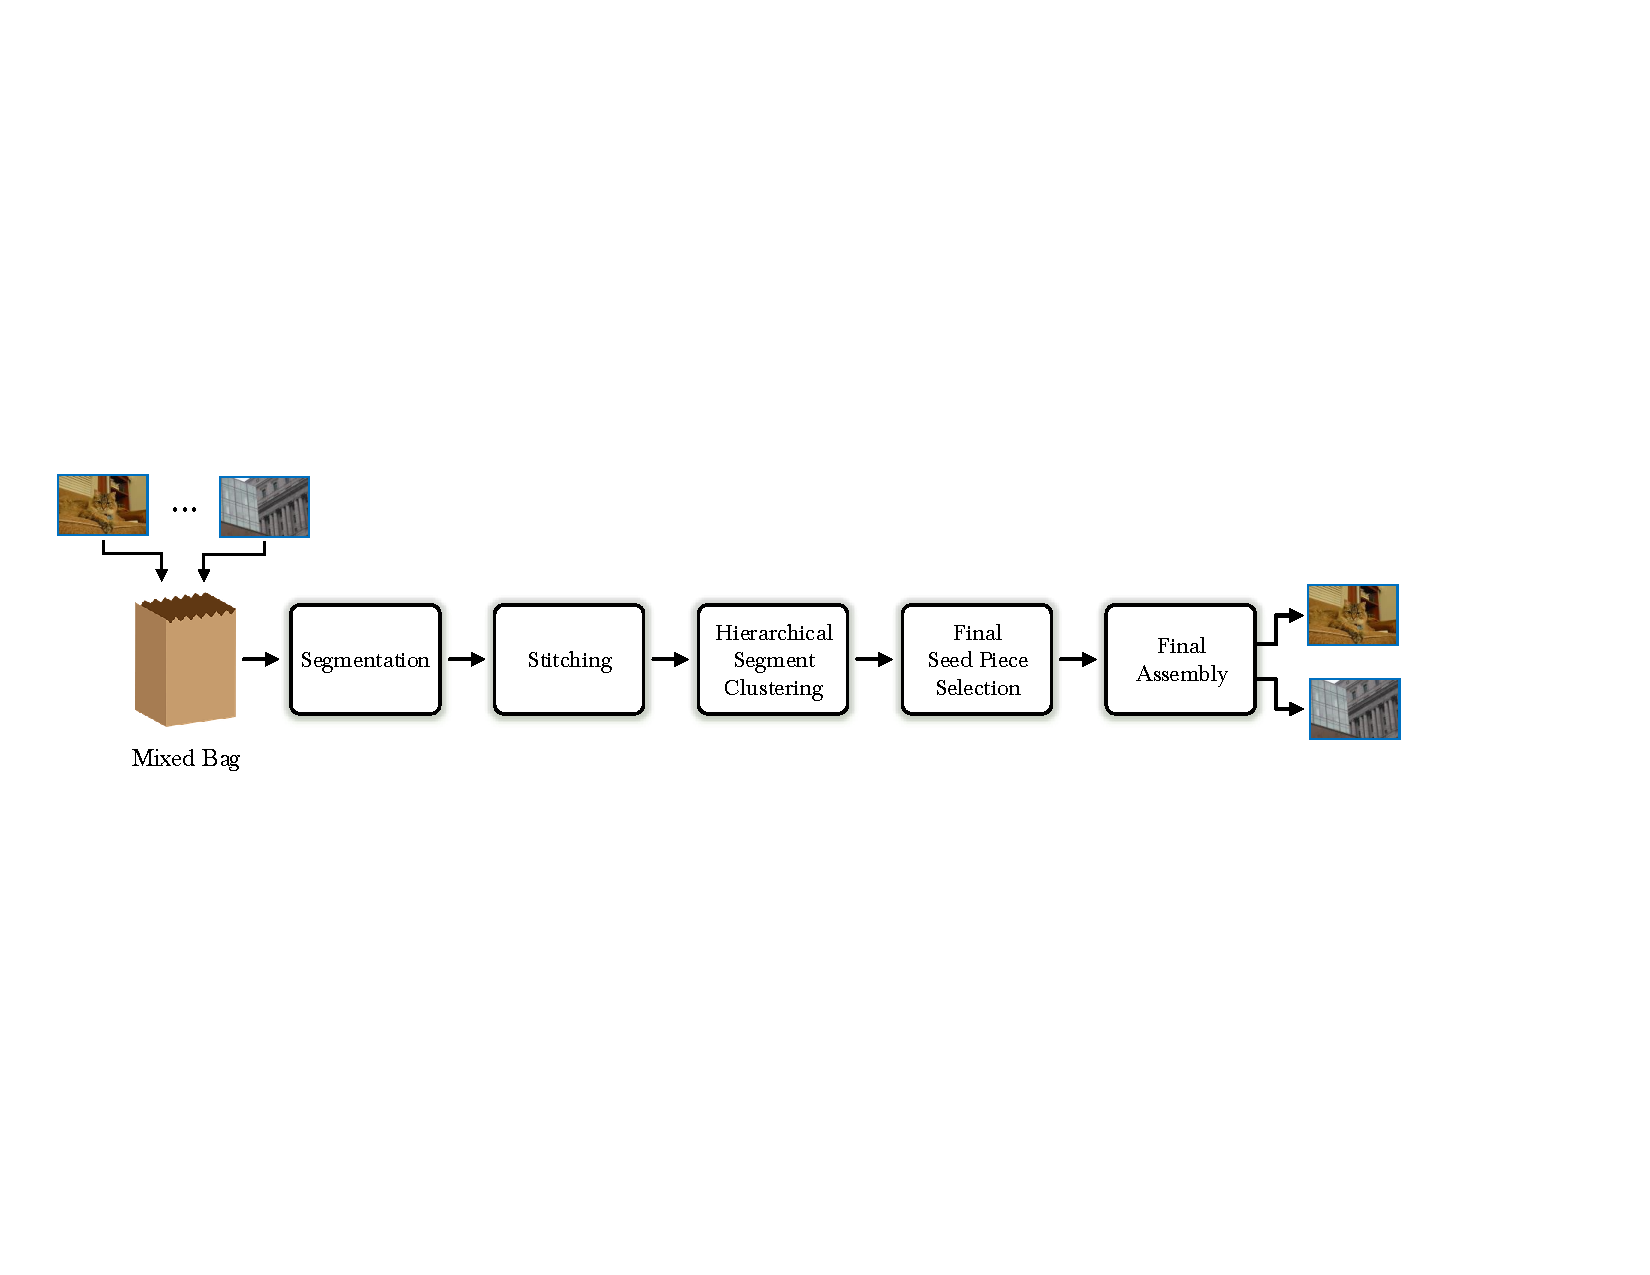
\includegraphics[width=1.0\textwidth]{images/cropped_algorithm_structure_overview.pdf}
	\caption{Components of the Mixed-Bag Puzzle Solver}\label{fig:multipuzzleSolverArchitecture}
\end{figure}

\begin{algorithm}[tb]
\caption{Pseudocode for the Mixed Bag Solver}\label{alg:mixedBagSolver}
\begin{algorithmic}[1]
\Function{MixedBagSolver}{$all\_pieces$}
    \State $solved\_segments \gets \textproc{Segmentation}\text{(} all\_pieces \text{)}$
	\State $overlap\_matrix \gets \textproc{Stitching}\text{(} solved\_segments \text{, } all\_pieces \text{)}$
	\State $clusters \gets \textproc{HierarchicalClustering} \text{(}solved\_segments \text{, } overlap\_matrix \text{)}$
	\State $puzzle\_start\_pieces \gets \textproc{FindStartingPieces} \text{(} clusters \text{)}$
	\State $solved\_puzzles \gets \textproc{RunFinalAssembly} \text{(} puzzle\_start\_pieces \text{, } all\_pieces \text{)}$
    \State \Return $solved\_puzzles$
\EndFunction
\end{algorithmic}
\end{algorithm}

\section{Assembler}\label{sec:SolverAssembler}

The assembler assigns the placement (and optionally rotation) of the puzzle pieces in the solved puzzle.  The Mixed-Bag Solver's architecture is largely independent of the particular assembler used.  Hence, any improvements or modifications to the assembler can be directly incorporated into the Mixed-Bag Solver to improve the solver's performance.  What is more, if a particular assembler performs better than others for a particular application, the assemblers can be interchanged.  This provides the Mixed-Bag Solver with significant flexibility and upgradability to maximize performance across a wide range of applications.

For all experiments in this thesis, the assembler proposed proposed by Paikin~\& Tal~\cite{paikin2015}.  As mentioned in Chapter~\ref{chap:previousWork}, their assembler is the current state of the art and is one of the few algorithms that natively supports Mixed-Bag puzzles.

\subsection{Assembler Time Complexity}


\subsection{Assembler Implementation}\label{sec:assemblerImplementation}

As of this publication, the implementation of Paikin~\&~Tal's algorithm is not open-source.  Hence, their algorithm was implemented as part of this thesis based off of the description in~\cite{paikin2015}.  This thesis' implementation is in the Python programming language and is fully open-source.

\section{Segmentation}\label{sec:Segmentation}

As detailed in Algorithm~\ref{alg:mixedBagSolver}, segmentation stages takes as input only the bag of puzzle pieces created from the original images; unlike all other solvers to date, this algorithm takes no other inputs.  The role of segmentation is to a basic provide structure to the unordered input.  This is done by partitioning the pieces into disjoint sets, referred to here as segments.  These segments are groups of puzzle pieces where there is a high degree of confidence that the pieces are assembled correctly.

Algorithm~\ref{alg:segmentation} outlines the basic segmentation framework; the implementation is iterative and will have one or more rounds.  In each round, all pieces not yet assigned to a saved segment are assembled as if they all belong to a single ground-truth image.  This strategy eliminates the need to make any assumptions regarding the input at this early stage.  What is more, it is expected that pieces from the same input puzzle may be assigned to multiple disjoint segments.  Section~\ref{sec:hierarchicalClustering} describes how these segments are merged using hierarchical clustering.

After the puzzle is assembled in a given round, the solved puzzle is then partitioned into segments; the segmentation procedure is described in Section~\ref{sec:segmentPuzzle}.  Assuming the largest segment exceeds the minimum allowed size\footnote{For this thesis, it was observed that a minimum segment size of 7 provided the best balance between solution quality and algorithm execution time.}, it is passed to the Stitching stage described in Section~\ref{sec:stitching}.  Similarly, the term ``\textit{$\alpha$}'' in Algorithm~\ref{alg:segmentation} dictates the segments in a given segmentation round, other than the largest one, that are also passed to the next stage of the Mixed-Bag Solver.  In this thesis, \textit{$\alpha$} was set to 0.5, meaning any segment that was at least half the size of the largest segment in that round is saved.  This scalar value provides sufficient balance between finding the largest possible segments for analysis and limiting overall execution time.

Once a piece is assigned to a saved segment, it is removed from the set of unassigned pieces.  Hence, those pieces will not be placed in the next segmentation round.  Segmentation continues until all pieces have been assigned to sufficiently large segments, or no segment exceeds the minimum allowed segment size.

\begin{algorithm}[tb]
\caption{Pseudocode for the Segmentation Algorithm}\label{alg:segmentation}
\begin{algorithmic}[1]
\Function{Segmentation}{$all\_pieces$}
    \State $saved\_segments \gets \{ \}$
    \State $unassigned\_pieces \gets \{ all\_pieces \}$
    \Loop
        \State $solved\_puzzle \gets \textproc{RunSinglePuzzleAssembly}(unassigned\_pieces)$
        \State $puzzle\_segments \gets \textproc{SegmentPuzzle}(solved\_puzzle)$
\item[]
        \State $max\_segment\_size \gets \text{maximum size of segment in } solved\_segments$
        \If{$max\_segment\_size \text{ < } smallest\_allowed$}
			\State \Return $saved\_segments$
        \EndIf
\item[]
        \ForEach{$segment \in puzzle\_segments$}
            \If{$|segment| \text{ > } \alpha \times max\_segment\_size$}
                \State $\text{add } segment \text{ to } saved\_segments$
                \State $\text{remove pieces in } segment \text{ from } unassigned\_pieces$
            \EndIf
        \EndFor
	\EndLoop
\EndFunction
\end{algorithmic}
\end{algorithm}

\subsection{The \textproc{SegmentPuzzle} Function}\label{sec:segmentPuzzle}

The \textproc{SegmentPuzzle} function shown in Algorithm~\ref{alg:segmentPuzzle} is adapted from the kernel growing segmentation procedure proposed by Pomeranz \textit{et al.}, where it was shown to have greater than 99.7\% accuracy identifying genuine neighbors \cite{pomeranz2011}. The kernel of each segment is a single seed piece.

\begin{algorithm}[tb]
\caption{Pseudocode to Segment a Solved Puzzle}\label{alg:segmentPuzzle}
\begin{algorithmic}[1]
\Function{SegmentPuzzle}{$solved\_puzzle$}
    \State $puzzle\_segments \gets \{ \}$
    \State $unassigned\_pieces \gets \{ \text{all pieces in } solved\_puzzle \}$
\item[]
    \While{$|unassigned\_pieces| \text{ > } 0$}
        \State $segment \gets \text{ new empty segment}$
        \State $seed\_piece \gets \text{next piece in } unassigned\_pieces$
        \State $queue \gets [seed\_piece]$
\item[]
        \While{$|queue| \text{ > } 0$}
            \State $piece \gets \text{next piece in } queue$
            \State $\text{add } piece \text{ to } segment$
\item[]
            \ForEach{$neighbor\_piece \text{ of } piece$}
            	\If{$\textproc{IsBestBuddies}(neighbor\_piece, piece)$}
            		\State $\text{add } neighbor\_piece \text{ to } \textit{queue}$
            		\State $\text{remove } neighbor\_piece \text{ from } unassigned\_pieces$
            	\EndIf
            \EndFor
        \EndWhile
\item[]
        \State $articulation\_points \gets \textproc{FindArticulationPoints}(segment)$
        \State $\text{remove } articulation\_points \text{ from } \textit{segment}$
\item[]
		\State $disconnected\_pieces \gets \textproc{FindDisconnectedPieces}(segment, seed\_piece)$ 
		\State $\text{remove } disconnected\_points \text{ from } segment$
\item[]
        \State $\text{add } \textit{articulation\_points} \text{ and } \textit{disconnected\_pieces} \text{ to } \textit{unassigned\_pieces}$               	
		\State $\text{add } segment \text{ to } puzzle\_segments$	
    \EndWhile
\item[]
    \State \Return $puzzle\_segments$
\EndFunction
\end{algorithmic}
\end{algorithm}

Whenever a piece is added to a segment, the algorithm examines all of the piece's neighbors.  Any of the adjacent pieces that satisfy the ``best buddy'' criteria as defined in Chapter~\ref{chap:previousWork} are also added to the segment.  This process continues until the segment has no neighboring best buddies. In Pomeranz \textit{et al.}'s algorithm, no changes were made to the segment after it reached the maximum size.  This approach can be sufficient when solving only a single puzzle at a time as they did.  However, it is common in Mixed-Bag puzzles that two or more correctly assembled segments are joined into a single cluster by very linking, usually in the form of narrow bridges no wider than a single piece.  These tenuous links are broken to prevent erroneous segment merging.  

\subsection{Articulation Points}\label{sec:ArticulationPoints}

A segment can be modeled as a graph with a single connected component.  The individual puzzle pieces represent the vertices while the edges are the interpiece best buddy relationships as defined in Chapter~\ref{chap:previousWork} and determined in Algorithm~\ref{} by the function ``\textproc{IsBestBuddies}''.  An articulation point is any vertex (i.e., puzzle piece) whose removal increases the number of connected components.  The Mixed-Bag Solver uses the algorithm proposed by \cite{cormenIntroToAlgorithms} for identifying articulation points.  While most implementations of this algorithm are recursive, this thesis instead uses an iterative approach as segment can be several thousand pieces in sizes.  As such, a recursive implementation is prone to stack overflows.

Any time an articulation point is removed, one or more pieces will necessarily become disconnected from the segment's seed.  Any such pieces are removed from the segment and returned to the set of unassigned pieces.  

\section{Stitching}\label{sec:stitching}

As discussed previously, a segment represents an ordering of pieces where there is a particularly high degree of confidence that the placement is correct.  In some areas of an image (e.g., a sky where there is little variation between pieces), the segmenter may not have high confidence that the puzzle is assembled correctly.  This often leads to a single ground-truth image being comprised of multiple segments. Since the Mixed-Bag Solver is not supplied with the number of input puzzles, it must quantify the extent to which any pairs of segments are related to ensure it can accurately estimate the number of ground-truth inputs.  

It is expected that two segments that were adjacent in their ground-truth image would eventually merge if one segment were allowed to expand. Since it is not known in which relative direction adjacent segment(s) may be located, the segment should be allowed to grow in all directions; however, the segment should not be forced to expand in a certain direction as it may lead to the formation of erroneous inter-segment coupling.  This concept serves the foundation of the inter-segment stitching used by the Mixed-Bag Solver.  The stitching process is described in the following subsections.

\subsection{Stitching Pieces}

As mentioned previously, a segment should be allowed, but not forced, to expand in all directions to try to identify related segments.  To achieve this, the Mixed-Bag Solver introduces the concept of a ``mini-assembly,'' which is similar to the standard assembly process described in Section~\ref{sec:SolverAssembler} with the expectation that it only places a limited number of pieces.\footnote{This thesis' implementation of the Mixed-Bag Solver uses 100 as the number of pieces placed during a mini-assembly.}  The seed piece of each of these assemblies is referred to as a ``stitching piece'' since they serve the role of ``stitching'' together associated segments.

\subsection{Stitching Piece Selection} 

Poor selection of stitching pieces can cause more subtle inter-segment links to be missed or lead to unnecessary execution time.  Algorithm~\ref{alg:selectStitchingPieces} outlines the procedure used by the Mixed-Bag Solver to select the stitching pieces.  It ensures that stitching pieces are sufficiently spaced from one another as well as from segment boundaries to minimize execution time while simultaneously ensuring sufficient coverage to detect subtle inter-segment relationships.  The following two subsections describe the two primary aspects of this algorithm, namely determining the distance of each piece to the nearest boundary as well as subpartitioning the segment for optimal inter-stitching piece spacing.

\begin{algorithm}[tb]
\caption{Pseudocode for Selecting the Stitching Pieces in a Segment}
\label{alg:selectStitchingPieces}
\begin{algorithmic}[1]
\Procedure{FindStitchingPieces}{$segment\_pieces$}
	\State $\textproc{FindPieceDistanceToOpen}(segment\_pieces)$
	\State $segment\_stitching\_pieces \gets \{ \}$
    \State $segment\_grid\_cells \gets \textproc{PartitionIntoGrid}(segment, grid\_cell\_width)$
	\ForEach{$grid\_cell \in segment\_grid\_cells$}
		\If{$\textproc{HasPieceAdjacentToOpen}(grid\_cell)$}
			\State $candidates \gets \text{set of pieces with } distance\_to\_open \text{ closest to target}$
			\State $stitching\_piece \gets piece \in candidates \text{ closest to center of } grid\_cell$
			\State $\text{add } stitching\_piece \text{ to } segment\_stitching\_pieces$
		\EndIf
	\EndFor
	\State \Return $segment\_stitching\_pieces$
\EndProcedure
\end{algorithmic}
\end{algorithm}


\subsubsection{Spacing between Stitching Pieces}\label{sec:spacingBetweenStitchingPieces}

If stitching pieces are too close together, the outputs from several mini-assemblers will be essentially identical.  In contrast, if stitching pieces are too far apart, the segment may not be able to grow towards any segments.

To address inter-stitching piece spacing, Algorithm~\ref{alg:selectStitchingPieces} sub-partitions each segment into a grid of adjacent regions.  The grid spans the entire segment starting from the piece in the upper left corner of the segment.\footnote{For this thesis, the target length and width of each grid cell was 10 pieces.}  As such, some grid cells along the right and bottom boundary of the segment will be narrower than the target grid cell width if the segment dimensions are not evenly divisible by the target. This grid system allows the algorithm to easily space out stitching pieces at some maximum spacing based off the grid cell width. 

Stitching pieces will only be selected from those grid cells that have at least one puzzle piece adjacent to an ``open location,'' which are all valid puzzle locations that has either a piece from a different segment or no piece at all. Section~\ref{sec:determiningSpacingToNearestOpenLocation} outlines the procedure used by the Mixed-Bag Solver to determine the distance each piece is from an open location.  Once this information has been found, finds the set of pieces (if any) who distance to the nearest open location matches the target value.  If no pieces satisfy that criteria, then the target value is decremented until at least one piece satisfies the criteria.     From amongst the pieces that matched the open location distance criteria, the piece that is closest to the center of the grid cell is selected as the stitching piece for that cell.  

\subsubsection{Spacing the Stitching Pieces from Open Locations}\label{sec:determiningSpacingToNearestOpenLocation}

It is not sufficient for stitching pieces to be placed solely around the external perimeter of a segment as it is common for segments to have internal where no pieces are present.  As such, stitching pieces are placed near all ``open locations,'' which are all valid puzzle locations that has either a piece from a different segment or no piece at all. 

If a stitching piece is too close to the edge of a segment, erroneous coupling between unrelated segments may occur.  To address this, Algorithm~\ref{alg:findDistanceToOpen} is used by the Mixed-Bag Solver to determine the distance between each piece in the segment and the nearest open location.  The algorithm follows an iterative boundary tracing technique; hence, during each iteration of the \textbf{while} loop on line~\ref{op:distanceRoundWhileLoop}, all segment pieces whose distance to the nearest open location is equal to $distance\_to\_open$ are explored.  Therefore, any pieces explored in the first iteration of the \textbf{while} loop would have a distance of 1 to the nearest open while those explored in the second iteration would have distance 2.  For this thesis, the target distance between a stitching piece and the nearest open location was 3; as explained in Section~\ref{sec:.

There are two primary reasons iterative boundary tracing was used for Algorithm~\ref{alg:findDistanceToOpen}.  First, the algorithm is robust enough to handle segment voids as well as potential necking within the segment where two large segment components are joined by a narrower bridge. What is more, since each piece is explored only once, the execution time of this algorithm is $O(n)$, where $n$ is the number of pieces in the segment.

\begin{algorithm}[tb]
\caption{Pseudocode for Determining a Segment Point's Manhattan Distance to the Nearest Open Location}\label{alg:findDistanceToOpen}
\begin{algorithmic}[1]
\Procedure{FindPieceDistanceToOpen}{$segment\_pieces$}
    \State $explored\_pieces \gets \{ \}$
    \State $locations\_at\_prev\_dist \gets \{ \text{all open locations adjacent to } segment\_pieces \}$
    \State $distance\_to\_open \gets 1$
\item[]
    \While{$|explored\_pieces| \text{ > } 0$} \label{op:distanceRoundWhileLoop}
        \State $locations\_at\_current\_dist \gets \{ \}$
\item[]
        \ForEach{$prev\_dist\_loc \in locations\_at\_prev\_dist$}
        	\ForEach{$adjacent\_loc \textbf{ of } prev\_dist\_loc$}
        		\If{$\exists \text{ } piece \text{ at }adjacent\_loc \textbf{ and } piece \notin explored\_pieces$}
        		
        			\State $\text{set } distance\_to\_open \text{ for } piece$
        			\State $\text{remove } piece \text{ from } explored\_pieces$
        			\State $\text{add } adjacent\_loc \text{ to } locations\_at\_current\_dist$
        		\EndIf
        	\EndFor
        \EndFor
\item[]
    \State $locations\_at\_prev\_dist \gets locations\_at\_current\_dist$
    \State $distance\_to\_open \gets distance\_to\_open + 1$
    \EndWhile
\EndProcedure
\end{algorithmic}
\end{algorithm}






\subsection{Quantifying Inter-Segment Relationships}

As mentioned previously, each segment, $\Phi_i$ will have one or more stitching pieces, $\zeta_x$, where $\zeta_x \in \Phi_i$.  Each stitching piece $\zeta_x$ for segment $\Phi_i$ will have a corresponding mini-solver output puzzle, $MS_{\zeta_x}$.  As each mini-solver is run, the solver output may grow towards neighboring segments.  If the solver output includes pieces from a different segment, there is a significantly increased likelihood the two segments came from the same input puzzle. 

Equation~\eref{eq:segmentOverlap} defines an overlap coefficient based on the mini-solver outputs to quantify the quantify the relationship between any two segments $\Phi_i$ and $\Phi_j$. The intersection between the mini-solver output and the corresponding segment needs to be normalized by the mini-solver's size.  It must also take into account the size of the corresponding segment since that can dictate in some cases dictate the maximum overlap if $|\Phi_j| < |MS_{\zeta_x}|$.

\begin{equation} \label{eq:segmentOverlap}
Overlap_{\Phi_i,\Phi_j} = \argmax_{\zeta_x \in \Phi_i} {\frac{|MS_{\zeta_x} \bigcap \Phi_j|}{\text{min}(|MS_{\zeta_x}|, |\Phi_j|)}}
\end{equation}

The mini-solver outputs will vary between segments based off their respective stitching piece selection as well as potentially the size of the segments.  Hence, in most cases, the overlap coefficient is asymmetric meaning that often $Overlap_{\Phi_i,\Phi_j} \neq Overlap_{\Phi_j,\Phi_i}$.  Section~\ref{sec:quantifyingSegmentSimilarity} defines how the overlap coefficients are normalized to quantify inter-segment similarity.

\section{Hierarchical Clustering of Segments}\label{{sec:hierarchicalClustering}}

Agglomerative hierarchical clustering is a bottom-up clustering algorithm where in each clustering round, two clusters are merged.  Algorithm~\ref{alg:hierarchicalClustering} shows the basic flow of the hierarchical clustering algorithm of the Mixed-Bag Solver; it is adapted from \cite{tanIntroToDataMining}.  

The only inputs to the hierarchical clustering algorithm are the segments found in the segmentation stage and the Segment Overlap Matrix from the Stitching stage.

\begin{algorithm}[tb]
\caption{Pseudocode for the Hierarchical Clustering of Segments}\label{alg:hierarchicalClustering}
\begin{algorithmic}[1]
\Function{HierarchicalClustering}{$solved\_segments, overlap\_matrix$}
	\State $\textit{segment\_clusters} = \{ \}$	
	\ForEach{$segment_i \in \textit{solved\_segments}$}
		\State $\text{add new segment cluster } \Phi_i \text{ containing } segment_i \text{ to } \textit{segment\_clusters}$
	\EndFor
\item[]
    \State $\text{Compute the similarity matrix } \Gamma \text{ from } overlap\_matrix$
\item[]
    \While{$\text{maximum similarity in } \Gamma \text{ > } \textit{min\_cluster\_similarity}$}
    	\State $\text{Merge the two most similar clusters } \Phi_i \text{ and } \Phi_j \text{ in } \textit{segment\_clusters}$
    	\State $\text{Update the similarity matrix, } \Gamma \text{ for the merged clusters}$
	\EndWhile
\item[]
    \State \Return $\textit{cluster\_segments}$
\EndFunction
\end{algorithmic}
\end{algorithm}

\subsection{Calculating the Initial Similarity Matrix}\label{sec:quantifyingSegmentSimilarity}

The Segment Overlap Matrix is a form of hollow matrix, where all elements in the matrix, except those along the diagonal, are populated with meaningful values.  In contrast, hierarchical clustering merges segments using a triangular, similarity matrix.  Equation~\eref{eq:segmentSimilarity} defines the similarity, $\omega_{i,j}$ between any two clusters $\Phi_i$ to $\Phi_j$.

\begin{equation} \label{eq:segmentSimilarity}
\omega_{i,j} = \frac{Overlap(\Phi_i, \Phi_j) + Overlap(\Phi_j, \Phi_i)}{2} 
\end{equation}

If there are $n$ solved segments found during segmentation, then the initial similarity matrix $\Gamma$ is size $n$ by $n$.  Each element in $\Gamma$ is defined by Equation~\eref{eq:similarityMatrix}.  Both $i$ and $j$ are bounded between $1$ and $n$ inclusive.  What is more, all elements in $\Gamma$ are normalized between 0 and 1, also inclusive.

\begin{equation} \label{eq:similarityMatrix}
\Gamma = \begin{cases} 
	0 & j >= i
\\
	\omega_{i,j} & i < j
\end{cases} 
\end{equation}

\subsection{Updating the Similarity Matrix via Single Linking}

The Mixed-Bag Solver uses the Single Link version of hierarchical clustering.  Hence, the similarity between any two cluster segments is defined as the similarity between the two most similar segments in either cluster.  This approach is required because two segments clusters may only be adjacent along the border of two of the composite segments.  

Equation~\eref{eq:segmentClusterMerge} defines the similarity between any a merged cluster containing segment clusters, $\Sigma_x$ and $\Sigma_y$, and any other segment cluster $\Sigma_z$.  Note that segment $\Phi_i$ is a member of the union of segment clusters $\Sigma_x$ and $\Sigma_y$ while segment $\Phi_j$ is a member of segment cluster $\Sigma_z$.

\begin{equation} \label{eq:segmentClusterMerge}
	\omega_{x \cup y,z} = \argmax_{\Phi_i \in (\Sigma_x \cup \Sigma_y)} \bigg( \argmax_{\Phi_j \in \Sigma_z} \omega_{i,j} \bigg) 
\end{equation}

\subsection{Terminating Hierarchical Clustering}

Unlike traditional hierarchical clustering, the Mixed-Bag Solver does not always continuing merging the segment clusters  until only a cluster remains. Rather, the solver continues clustering until the maximum similarity between any of the remaining clusters drops below a predefined threshold.  In this thesis, a minimum inter-cluster similarity of $0.1$ provided sufficient clustering accuracy without merging unrelated segments.

The number of segments clusters remaining at the end of hierarchical clustering represents the expected number of ground-truth images provided to the solver.  The segment clusters are then passed to the next stage to determine the final seed pieces for each output puzzle.

\section{Final Seed Piece Selection}\label{sec:finalSeedPiece}

Most of the modern jigsaw puzzle solvers \cite{pomeranz2011, sholomon2013, paikin2015} rely on a kernel growing model, where a kernel is a partial assembly of one or more pieces.  As such, once the Mixed-Bag Solver has determined the expected number of input puzzles via hierarchical clustering, the algorithm then selects the seed piece for each of the output solutions. 

In Chapter~\ref{chap:previousWork}, it was explained that Paikin~\& Tal select a piece as an output puzzle's seed if seed piece to be the ``is both distinctive and lies in a distinctive region.''  They apply this criteria greedily during runtime.  Hence, their algorithm often picks suboptimal seeds (e.g., pieces from the same input puzzle are selected as seeds for multiple output puzzles).  In contrast, the combination of segmentation and hierarchical clustering in the Mixed-Bag Solver partitions the set of input pieces into disjoint sets, with each set roughly approximating a single solved puzzle.  Therefore, the Mixed-Bag Solver selects the seed for each output puzzle from the members of its associated segment cluster.  The algorithm uses the same approach as Paikin~\& Tal wherein the selected seed from the segment cluster is a ``piece that is both distinctive and lies in a distinctive region.''  However, since this selection is not made greedily and instead uses the segment clusters, the quality of the selection is superior.

\section{Final Assembly}